\documentclass[]{IEEEtran}
% some very useful LaTeX packages include:
%\usepackage{cite}      
\usepackage{graphicx}   
\usepackage{subfigure} 
\usepackage{url}       
\usepackage{amsmath}    
\usepackage{caption2}
% Your document starts here!
\begin{document}

% Define document title and author
	\title{Weekly Report}
	\author{Adviser: Prof. Yang Wen \\Student: Cheng Wensheng\\ Period: 2018.9.23-9.30
	}
	\markboth{Visual Information Processing Group}{}
	\maketitle

% Write abstract here
\begin{abstract}
	This week I mainly put my effort on dealing with the SAR image of Shang Hai and writing project application plan.
\end{abstract}

% Each section begins with a \section{title} command
\section{Sar contest}
	% \PARstart{}{} creates a tall first letter for this first paragraph
	\PARstart{T}{his} week I processed images labeled by junior students before and tested with basic semantic segmentation nets.
	\begin{itemize}
		\item The SAR images of Shang Hai city have lower resolution than those in the SAR contest, and the background is more complex than those in contest. The category of things in the images of SAR contest is less than images of Shang Hai and the boundry of the former is clearer than the latter. 
		\item I tried RefineNet, and the F1 score is about 55\%. To write papers based on this, I need to improve the accuracy and compare it with those traditional algorithms.
		    
	\end{itemize}
	
	Fig.~\ref{fig:fw} is the optical image. Fig.~\ref{fig:rt} is the SAR image. Fig.~\ref{fig:gt} is the ground truth. Fig.~\ref{fig:out} is the predicted image.

\section{Project plan}
% \PARstart{}{} creates a tall first letter for this first paragraph
\PARstart{A}{bout} the project plan, with the arrangement of Guo Wei, I'm in charge of the research goal, content and key problems.
\begin{itemize}
	\item Since research goal and research content are pointed out in the guidance file, I add corresponding content according to the files written by Yu Huai.
	\item We need to finish the file before Oct, 9th. Then we would adjust the content with the opinions of Prof. Yang and hand in this. 
	
\end{itemize}


\newpage


\begin{figure}
	\vspace{2.5cm}
	\begin{minipage}[t]{0.5\linewidth}
		\centering
		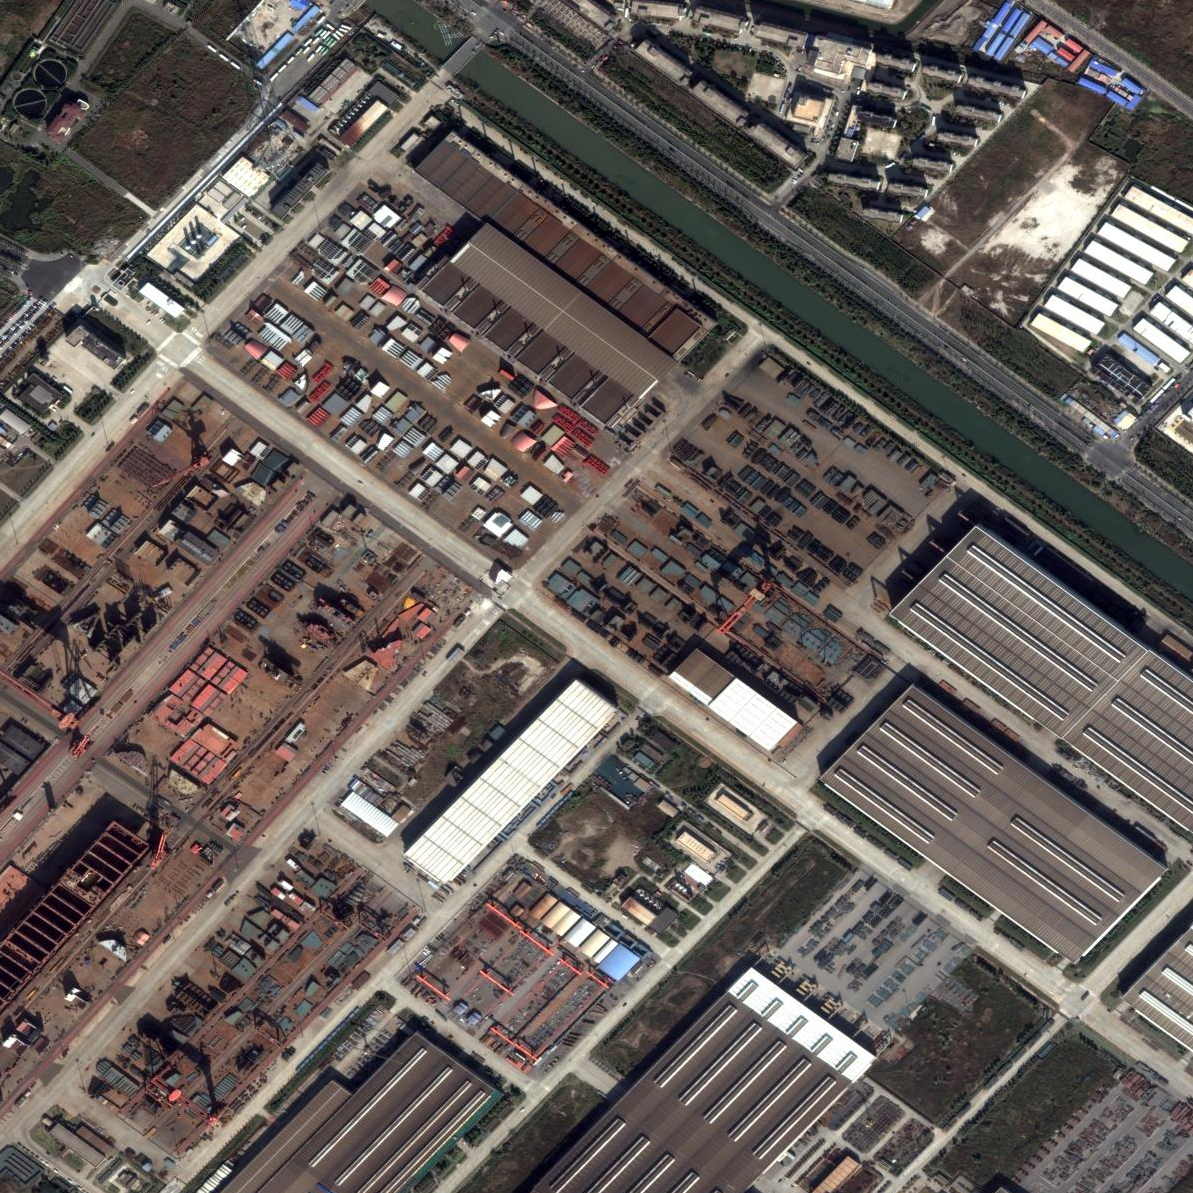
\includegraphics[width=0.9\columnwidth]{fw}
		\caption{Optical image}
		\label{fig:fw}
	\end{minipage}%
	\begin{minipage}[t]{0.5\linewidth}
		\centering
		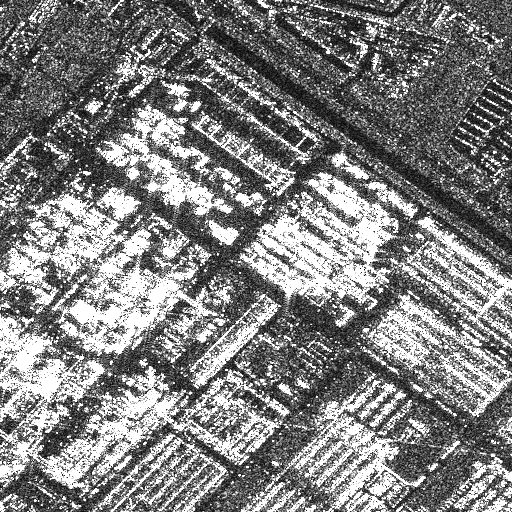
\includegraphics[width=0.9\columnwidth]{rt}
		\caption{SAR image}
		\label{fig:rt}
	\end{minipage}
\end{figure}

\begin{figure}
	%	\vspace{2.5cm}
	\begin{minipage}[t]{0.5\linewidth}
		\centering
		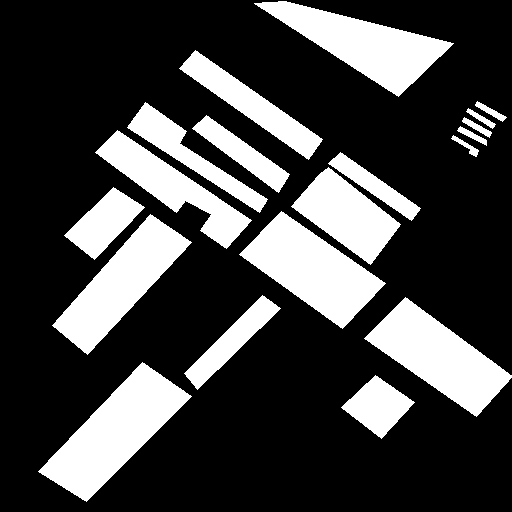
\includegraphics[width=0.9\columnwidth]{SAR01-00171_gt}
		\caption{Ground truth}
		\label{fig:gt}
	\end{minipage}%
	\begin{minipage}[t]{0.5\linewidth}
		\centering
		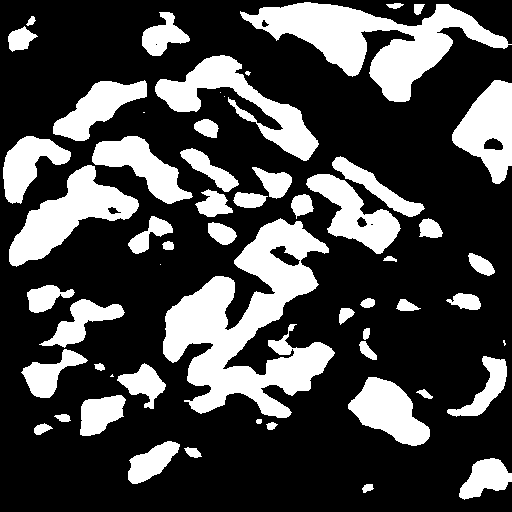
\includegraphics[width=0.9\columnwidth]{SAR01-00171_pred}
		\caption{Output image}
		\label{fig:out}
	\end{minipage}
\end{figure}


%\begin{figure}[!hbt]
%%		 Center the figure.
%		\vspace{0.7cm}
%%		\hspace{50cm}
%		\begin{center}
%			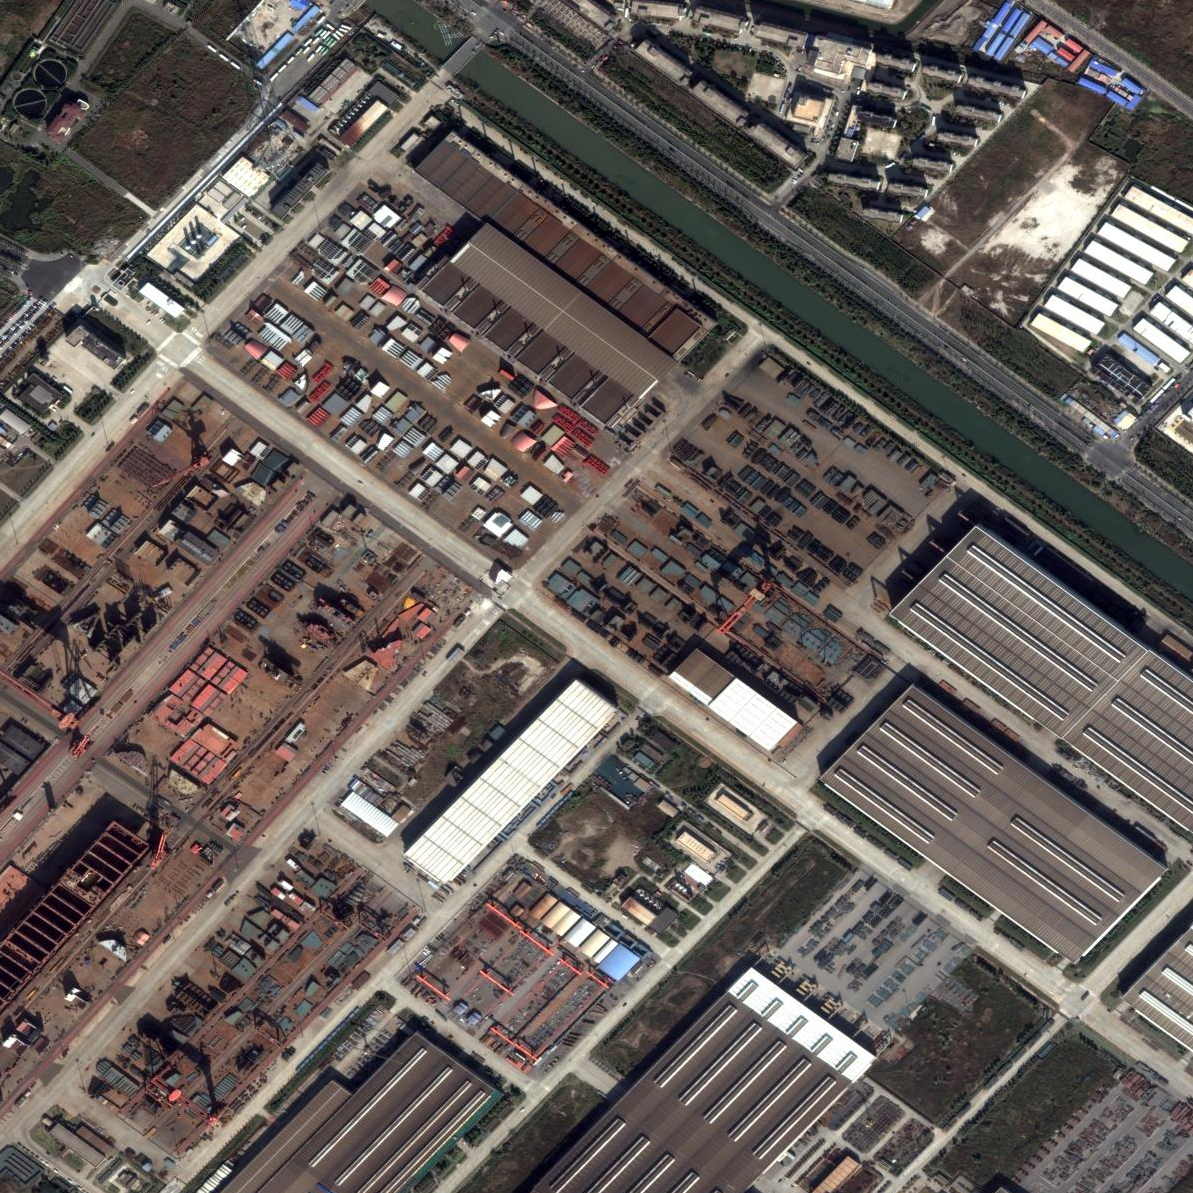
\includegraphics[width=0.2\columnwidth]{fw}
%				%		 Create a subtitle for the figure.
%			\caption{CNN methods result}
%			\label{fig:fw}
%		    \vspace{0.2cm}
%			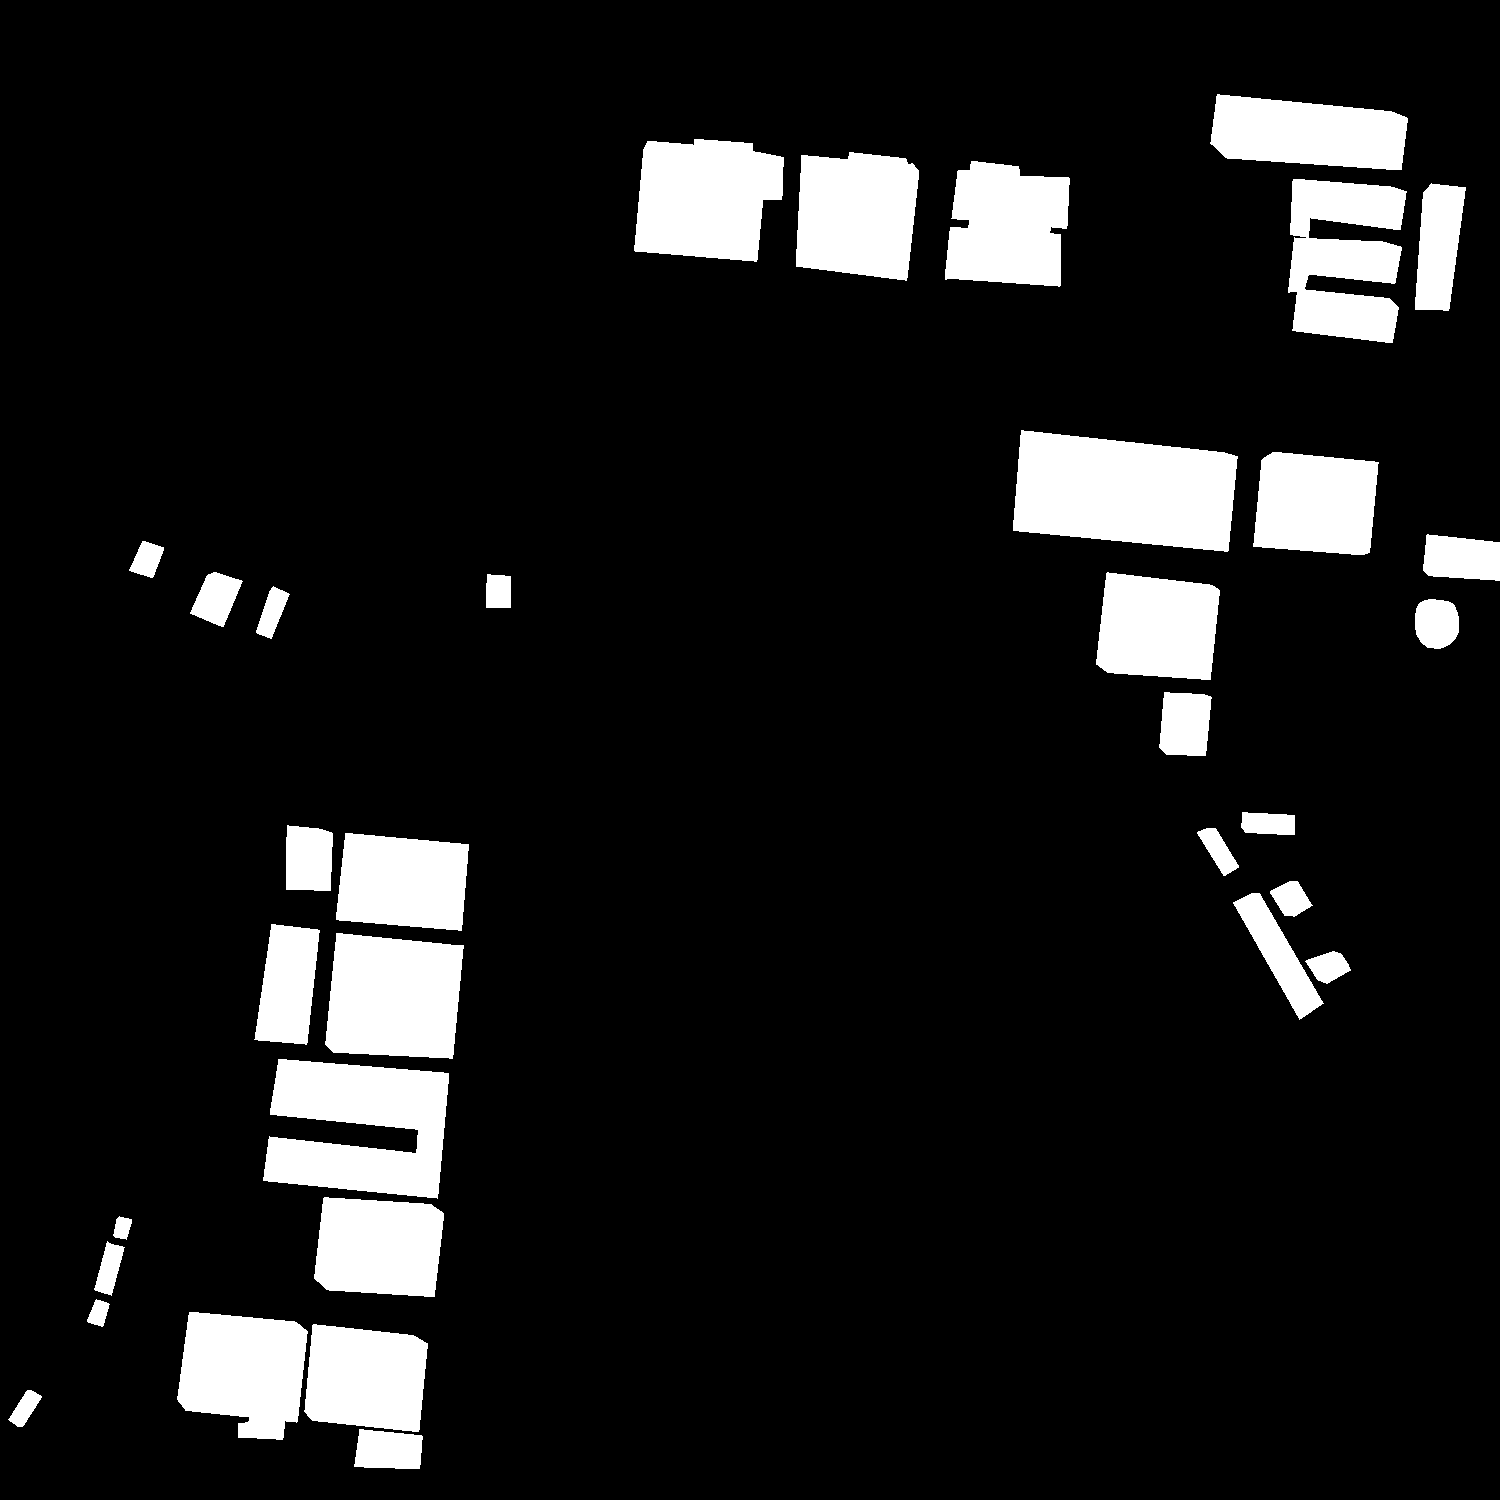
\includegraphics[width=0.2\columnwidth]{rs}
%				%Create a subtitle for the figure.
%			\caption{Ground truth}
%			\label{fig:rt}
%		\end{center}
%	\end{figure}



% Your document ends here!
\end{document}